\begin{figure}[h]
\centering
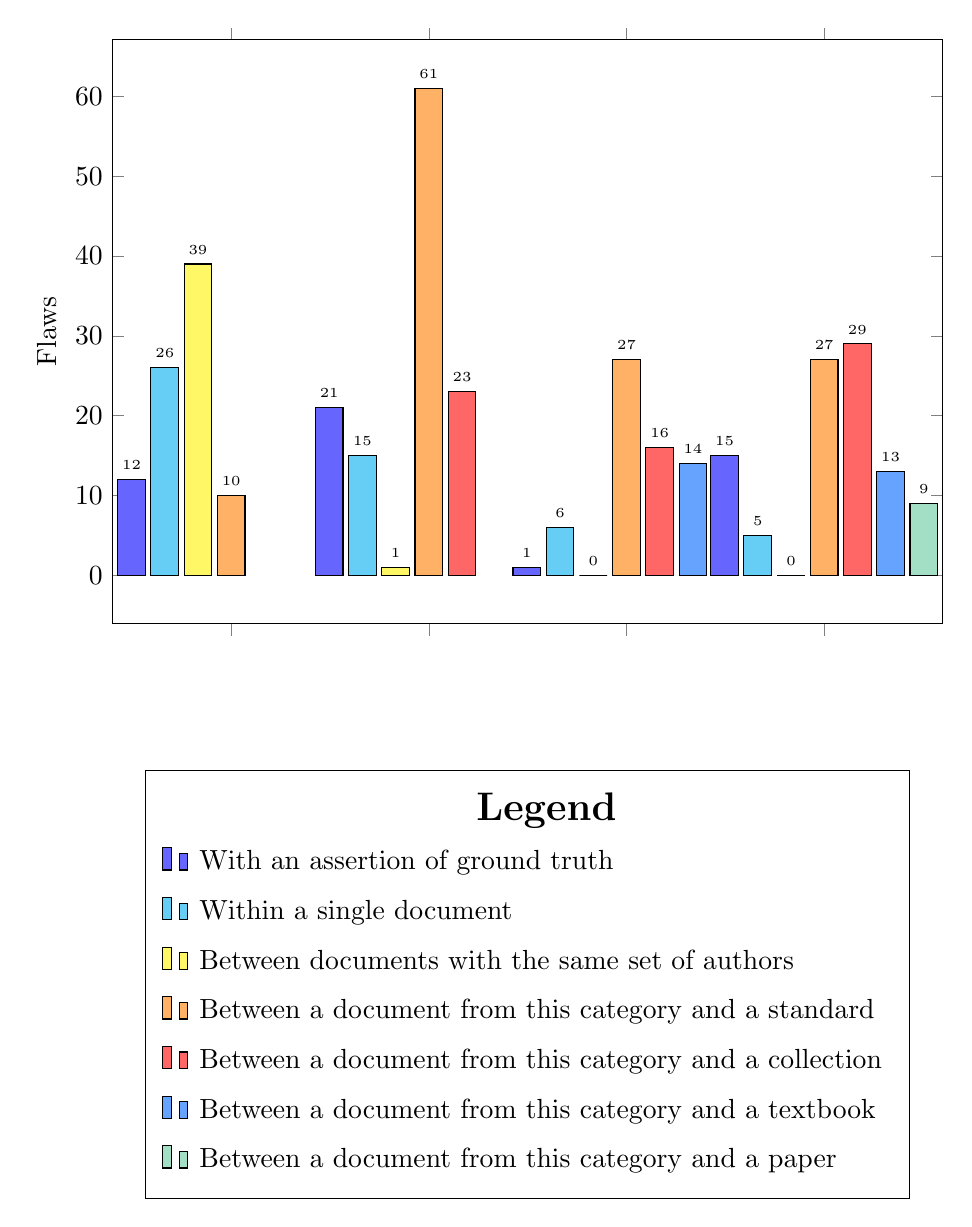
\begin{tikzpicture}
\begin{axis}[
width=\textwidth, height=9cm,
symbolic x coords={std,meta,text,paper},
xtick=data,
xticklabels={{\parbox{0.16\textwidth}{\centering \stds{}}},{\parbox{0.16\textwidth}{\centering \metas{}}},{\parbox{0.16\textwidth}{\centering \texts{}}},{\parbox{0.16\textwidth}{\centering \papers{}}}},
ylabel=Flaws, ybar,
enlargelimits=0.2, enlarge y limits=0.1,
legend style={at={(0.5,-0.25)}, anchor=north, legend columns=1,
inner xsep=6pt,inner ysep=4pt,
nodes={inner sep=4pt,text depth=0.3em},},
legend cell align=left,
nodes near coords,
every node near coord/.append style={font=\tiny},
]
\addlegendimage{empty legend}
\addplot[fill=blue!60] coordinates {(std, 12) (meta, 21) (text, 1) (paper, 15)};
\addplot[fill=cyan!60] coordinates {(std, 26) (meta, 15) (text, 6) (paper, 5)};
\addplot[fill=yellow!60] coordinates {(std, 39) (meta, 1) (text, 0) (paper, 0)};
\addplot[fill=orange!60] coordinates {(std, 10) (meta, 61) (text, 27) (paper, 27)};
\addplot[fill=red!60] coordinates {(meta, 23) (text, 16) (paper, 29)};
\addplot[fill=blue!60!cyan!60] coordinates {(text, 14) (paper, 13)};
\addplot[fill=cyan!60!yellow!60] coordinates {(paper, 9)};
\legend{\hspace{3.4cm} \Large \textbf{Legend},With an assertion of ground truth,Within a single document,Between documents with the same set of authors,Between a document from this category and a standard,Between a document from this category and a collection,Between a document from this category and a textbook,Between a document from this category and a paper}
\end{axis}
\end{tikzpicture}
\caption{Identified flaws by the source tier responsible. Some bars are omitted as they correspond to comparisons we do not make; see \Cref{flaw-cred-compare}.}\label{fig:flawBars}
\end{figure}
